\documentclass[titlepage]{jarticle}
\usepackage{h31ec-exp}
\usepackage[yen]{okuverb}
\usepackage[dvipdfmx]{graphicx}

\title{{\TeX}によるレポート作成}
\grade{3年32番}
\author{平田 蓮}
\team{}
\date{2019年5月10日}
\expdate{2019年4月8日,4月15日, 4月22日, 5月9日}
\coauthor{}

\begin{document}
\maketitle
\section{はじめに}
	本実験では, ~組版ソフトウェアの{\TeX}を用いて, ~学生実験などのレポートを作成する方法を学ぶ.
	~本実験を進めるにあたり, ~レポートを作成するうえで注意すべきことを理解しておく必要がある.

	以下, ~{\TeX}の機能を順に練習していく.

\section{基本練習}
	節, ~小節, ~小小節には自動的に番号が付けられる.
	\subsection{段落の分け方}
		本文の段落を変えるには, ~空行を入れればよい.

		日本語文章の場合, ~段落の最初の1文字分が自動的に字下げされる. \\
		強制改行をすると, ~この行のように字下げが行われない. ~したがって,
		~強制改行を段落の区切りに使ってはいけない.

	\subsection{文字サイズの変更}\label{sec:文字サイズ}
		{\TeX}では標準で10種類の文字サイズが使える. ~たとえば, ~{\footnotesize 脚注の文字サイズ	(footnotesize)}
		{\small ちょっと小さい字 (small)}{\large ちょっと大きい字 (large)}のようにサイズを変えて表示できる.

	\subsection{記号}
		いくつかの文字はそのままでは出力できないので, ~特別な書き方をする. \# \& \% \& \_ \~{} \{ \}

		``引用記号''には, ~ダブルォオーテーションは使わず,
		~``バッククォート(Shift+@)''と``クォーテーション(Shift+7)''を2連で使う.

	\subsection{環境}
		さまざまな文書形式は「環境」で提供される. ~環境とは,
		~\verb|\begin{環境名}|で始まり, ~\verb|\end{環境名}|で終わるものである.

		\subsubsection{箇条書き}
			文章中で事柄を列挙するときに使われる箇条書きの形式には, ~番号付き箇条書き, ~ 番号なし箇条書き,
			~見出し付き箇条書きの3種類がある.

			\paragraph{番号付き箇条書き}
			\begin{enumerate}
				\item 項目1
				\item 項目2
			\end{enumerate}

			\paragraph{番号なし箇条書き}
			\begin{itemize}
				\item 項目1
				\item 項目2
			\end{itemize}

		\subsubsection{揃え}
			文字揃えもよく使う機能である. ~左揃え, ~中央揃え, ~右揃えの3種類がある.

			\begin{center}
				中央揃え
			\end{center}

			\begin{flushright}
				右揃え \\
				複数行記述するときは, ~強制改行を使う
			\end{flushright}

		\subsubsection{その他の環境}
			そのまま出力するverbatim環境は, ~プログラムをそのまま載せたいときなどに便利である.

			\begin{verbatim*}
				#include <stdio.h>
				int main(void) {
				  printf("Hello, world!\n");
				  return 0;
				}
			\end{verbatim*}

			verbatim環境使用時の注意点としては, ~TAB文字は切り捨てられるため,
			~字下げの空白がTAB文字で入力されている場合は, ~半角スペースで置き換える必要があることである.

	\subsection{相互参照}
		レポートで特に便利なのは, ~\verb|\label|コマンドと\verb|\ref|,
		\verb|\pageref|コマンドを用いた相互参照である. ~節や図, ~表, ~式の番号を本文中で参照したいときに,
		~参照したい式などの直後にラベルを定義しておけば, ~本文中でそのラベルを参照するだけで,
		~対応する番号を自動的に挿入することができる.

	\paragraph{相互参照の練習:}
	文字サイズの変更については, ~第\ref{sec:文字サイズ}節で練習した(1ページ).

	なお, ~相互参照を使っているときには, ~ラベルに変更があると, ~2回コンパイルをする必要がある.


\section{数式の練習}
	本文中の式番号の参照も, ~相互参照の機能を使う. ~これにより, ~文章の順番を入れ替えた場合でも自動的に式番号が
	振り直され, ~正しい式番号が参照される.

	\subsection{基本練習}
		\subsubsection{本文中の数式}
			関数$y = ax^2 + bx + c$を描く.

		\subsubsection{別行立て数式}
			\paragraph{1行, ~式番号付き}
			\begin{equation}
				y = ax^2 + bx + c
			\end{equation}

			\paragraph{複数行, ~式番号付き}
			\begin{eqnarray}
				y &=& ax^2 + bx + c \\
				x + y &<& -4 \nonumber
			\end{eqnarray}

			式の最後に\verb|\nonumber|を書くことで, ~一部の式に番号を付けないようにもできる.

	\subsection{数式の記述練習}
		式(\ref{eqn:2乗})と式(\ref{eqn:3乗})は, ~式の変形の公式である.
		\begin{eqnarray}
			(a \pm b)^2 &=& a^2 \pm 2ab + b^2 \label{eqn:2乗} \\
			(a \pm b)^3 &=& a^3 \pm 3a^2b + 3ab^2 \pm b^3 \label{eqn:3乗}
		\end{eqnarray}

		式(\ref{eqn:加法定理})は, ~三角関数の加法定理の公式である.
		\begin{eqnarray}
			\sin(\alpha \pm \beta) &=& \sin{\alpha}\cos{\beta} \pm \cos{\alpha}\sin{\beta}\label{eqn:加法定理}
		\end{eqnarray}

		式(\ref{eqn:定積分})は, ~定積分の性質を表している.
		\begin{equation}
			\int_a^b kf(x)dx = k\int_a^b f(x)dx \;(kは定数)\label{eqn:定積分}
		\end{equation}

		次に, ~一般の2次方程式の解の公式を導出する. ~2次方程式
		\begin{equation}
			ax^2 + bx + c = 0 \label{eqn:2次方程式}
		\end{equation}
		\\
		の両辺を$x^2$の係数$a$で割って, ~定数項を右辺に移項すれば,
		$$
			x^2 + \frac{b}{a}x = - \frac{c}{a}
		$$
		となる. ~さて, ~左辺に完全平方式を作るために, ~両辺に$\displaystyle \left(\frac{b}{2a}\right)^2$を加えれば,
		\begin{eqnarray*}
			x^2 + 2 \cdot \frac{b}{2a}x + \left(\frac{b}{2a}\right)^2 &=& \left(\frac{b}{2a}\right)^2 - \frac{c}{a} \\
			\left(x + \frac{b}{2a}\right)^2 &=& \frac{b^2 - 4ac}{4a^2}
		\end{eqnarray*}
		となる. ~したがって, ~両辺の平方根を作れば,
		\begin{eqnarray}
			x + \frac{b}{2a} &=& \pm\frac{\sqrt{b^2 - 4ac}}{2a} \nonumber \\
			x &=& \frac{-b \pm \sqrt{b^2 - 4ac}}{2a} \label{eqn:解の公式}
		\end{eqnarray}
		これが, ~式(\ref{eqn:2次方程式})の解を与える公式である. ~しかしながら, ~上の計算は, ~$D = b^2 - 4ac \geq$
		であるときに成り立つ. ~しかし, ~複素数を用いれば, ~$D = b^2 - 4ac < 0$の場合にも,
		~式(\ref{eqn:解の公式})は解の公式となる.


\section{図と表の練習}
	ここでは, ~これまでの実験レポートで扱った内容を題材に, ~図と表の作成と, {\TeX}文書への挿入について練習する.

	図については, ~PowerPointを用いて図を作成し, ~Metafile to EPS Converterを用いて, ~EPSファイルに変換して
	~文書に挿入する方法を習得する.

	表については, ~table環境およびtabular環境を用いて計測データの表を作成する手順を習得する.

	さらに, ~Excelを用いてグラフを作成し, ~ そのグラフをMetafile to EPS Converterを用いてEPSファイルに
	変換し, ~文書に挿入する方法を修得する.

	\subsection{実験内容}
		図\ref{fig:実験回路}は, ~オームの法則の実験回路である. ~この回路を用いて, ~一定電圧下で負荷抵抗の値を
		増加させたときの電流値を測定する.

	\subsection{実験結果}
		前節の実験の結果を表\ref{tab:電流値の測定結果}に示す.

		表\ref{tab:電流値の測定結果}をグラフに表すと図\ref{fig:抵抗-電流グラフ}のようになる.

		グラフから, ~電圧が一定の条件下では, ~電流値は抵抗値に反比例していることがわかる.

	\begin{figure}[h]
		\center{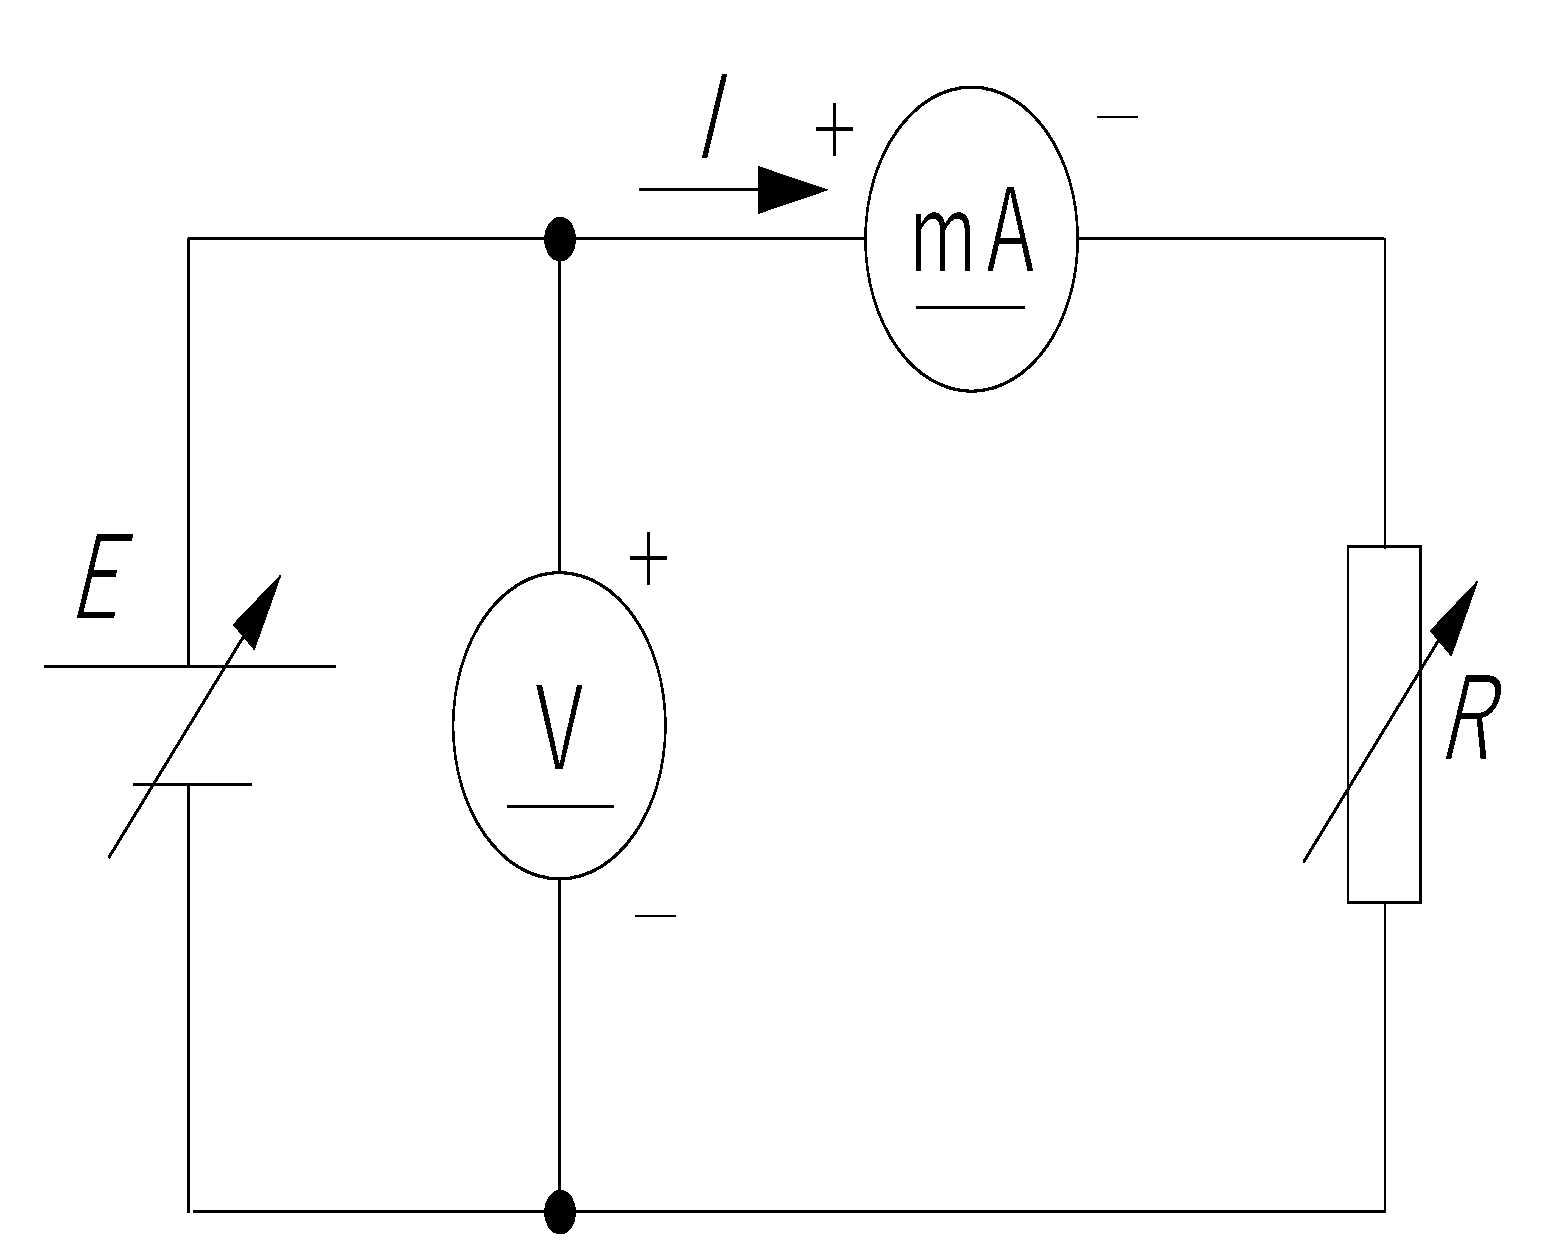
\includegraphics[width=8cm, height=4.5cm]{jikkennkairo.eps}}
		\caption{実験回路} \label{fig:実験回路}
	\end{figure}

	\begin{table}[h]
		\caption{電流値の測定結果} \label{tab:電流値の測定結果}
		\begin{center}
		\renewcommand{\arraystretch}{0.7}
		\begin{tabular}{r||r|r||r|r} \hline
			\multicolumn{1}{c||}{印加電圧} & \multicolumn{2}{c||}{5[V]} & \multicolumn{2}{c}{10[V]}\\ \hline
			\multicolumn{1}{c||}{負荷抵抗[k$\Omega$]} &
			\multicolumn{1}{c|}{理論値[mA]} & \multicolumn{1}{c||}{実測値[mA]} &
			\multicolumn{1}{c|}{理論値[mA]} & \multicolumn{1}{c}{実測値[mA]}\\ \hline
			0.1 & 50.0 & 49.9 & 100.0 & 99.1 \\
			0.2 & 25.0 & 24.1 &  50.0 & 49.9 \\
			0.3 & 16.7 & 16.5 &  33.3 & 32.5 \\
			0.4 & 12.5 & 12.5 &  25.0 & 24.3 \\
			0.5 & 10.0 & 10.0 &  20.0 & 20.0 \\
			0.6 &  8.3 &  8.4 &  16.7 & 16.2 \\
			0.7 &  7.1 &  7.1 &  14.3 & 14.3 \\
			0.8 &  6.3 &  6.2 &  12.5 & 12.5 \\
			0.9 &  5.6 &  5.6 &  11.1 & 11.1 \\
			1.0 &  5.0 &  5.0 &  10.0 &  9.9 \\ \hline
		\end{tabular}
		\end{center}
	\end{table}

	\begin{figure}[h!]
		\center{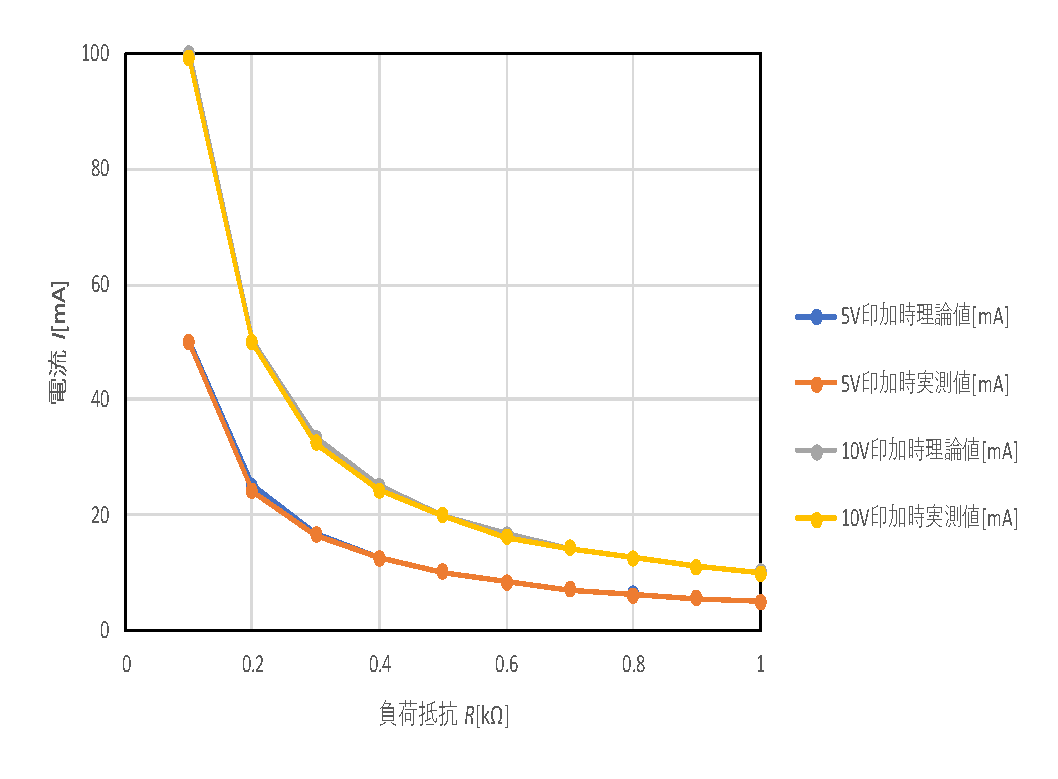
\includegraphics[width=15cm, height=8cm]{graph.eps}}
		\caption{抵抗-電流グラフ} \label{fig:抵抗-電流グラフ}
	\end{figure}

	\subsection{画像ファイルの挿入}
		{\TeX}文書には, ~図\ref{fig:画像の挿入例}のように画像ファイルを挿入することも可能である.


		\begin{figure}[h]
			\center{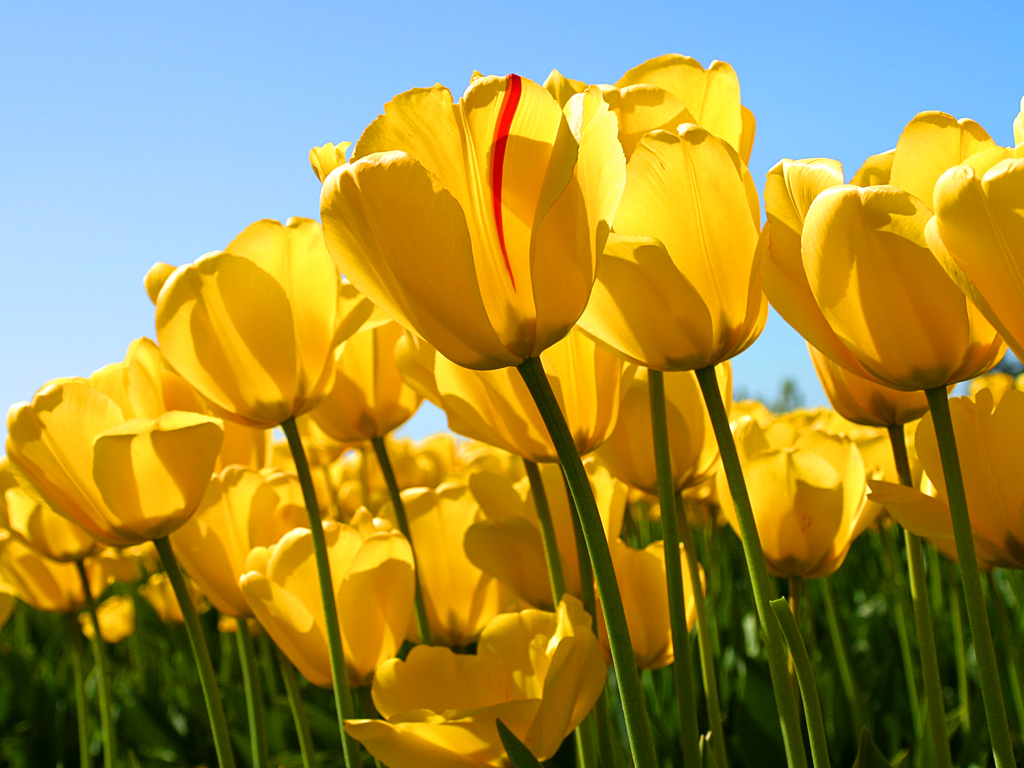
\includegraphics[width=6cm]{hana.png}}
			\caption{画像の挿入例} \label{fig:画像の挿入例}
		\end{figure}

\section{考察}
	\subsection{WordのようなWYSIWYG形式のソフトウェアによる文書作成と,
				~{\TeX}のようなマークアップ言語による文書作成の比較}
		Wordなどのソフトウェアと比べて, ~{\TeX}を使うことによって, ~レイアウトを考える手間が省けた.
		~Wordを使用した場合, ~章や節の番号をつける際に手動で入力し, ~位置を調節しないといけない.
		~それによって無駄に時間を使ってしまったことが一年生のころにあり, ~私はそれから{\TeX}を使い始めた.

		また, ~{\TeX}の欠点として, ~「コンピュータ任せ過ぎる」というものがある.
		~{\TeX}では, ~レイアウトをすべてコンピュータに任せて作成するので, ~特に図を入れる時などに, ~融通が
		利かないことがある. ~今回のから例を挙げると, ~5ページ目に図二つと表を入れる時に,
		~うまく収まるように画像のサイズ変換を何回も行った. ~これもやりやすくするような方法があるかもしれないが,
		~とりあえず, ~今回は少し面倒に感じた.

		去年の後期はレポート課題がなく, ~{\TeX}に触らない期間が半年ほどあったが, ~今回の演習を通してそれなりに
		思い出すことができた. ~ページ分割のような, ~さらに高度な{\TeX}技術もまた使いこなせるようになりたい.


	\subsection{実験テキストに盛り込むべき事項, ~説明が不十分と思われる個所について}
		まず, ~箇条書きの説明が書いてある6ページで, ~箇条書きのコードに, ~出力例を添えてあると学生から見ても
		直観的でどのような形式になるのかが見てわかりやすくなるかと感じた.

		また, ~13ページの{\ttyen}tabular環境と{\ttyen}multicolumn環境の列指定の説明にて,
		~縦棒の説明が少し不十分に感じた. ~先生の説明と併せて聞いていると理解できたが,
		~聞き逃してしまった場合など, ~察しが良い学生以外は詰まりやすいと思った.
		~{\ttyen}multicolumnの列指定の部分で, ~隣り合う{\ttyen}multicolumnの共通部分で罫線を
		指定してしまうと重複が起きることなども書いてあるとよいと思う.

		最後に, ~これは内容の不足ではなく, ~書いてある順番の話だが, ~10ページから書いてある記号一覧は,
		~9ページの添え字の解説より前に書いてあったほうが, ~学生の目につきやすいと感じた. ~これは一概にテキストが
		悪いとは言えないが, ~ギリシャ文字はどう描くのかと近くの席の3人ほどに聞かれたので,
		~10ページにあると見逃がしやすいのかもしれない.

\begin{thebibliography}{1}
	\bibitem{竹部} 竹部啓輔,「{\TeX}によるレポート作成」, ~平成31年度電子制御工学実験 - 3年前期テキスト
		pp.A-1-A-18 (2019/4).
\end{thebibliography}
\end{document}
